%%
%% Frame 1
%%
%\begin{frame}[t]{Foundations for Future Work}
%\vspace{-3ex}
%\begin{center}
%\only<1>{\hh{First Order Logic} \hspace{10ex} \hh{Lexical Methods} \\}
%\only<1>{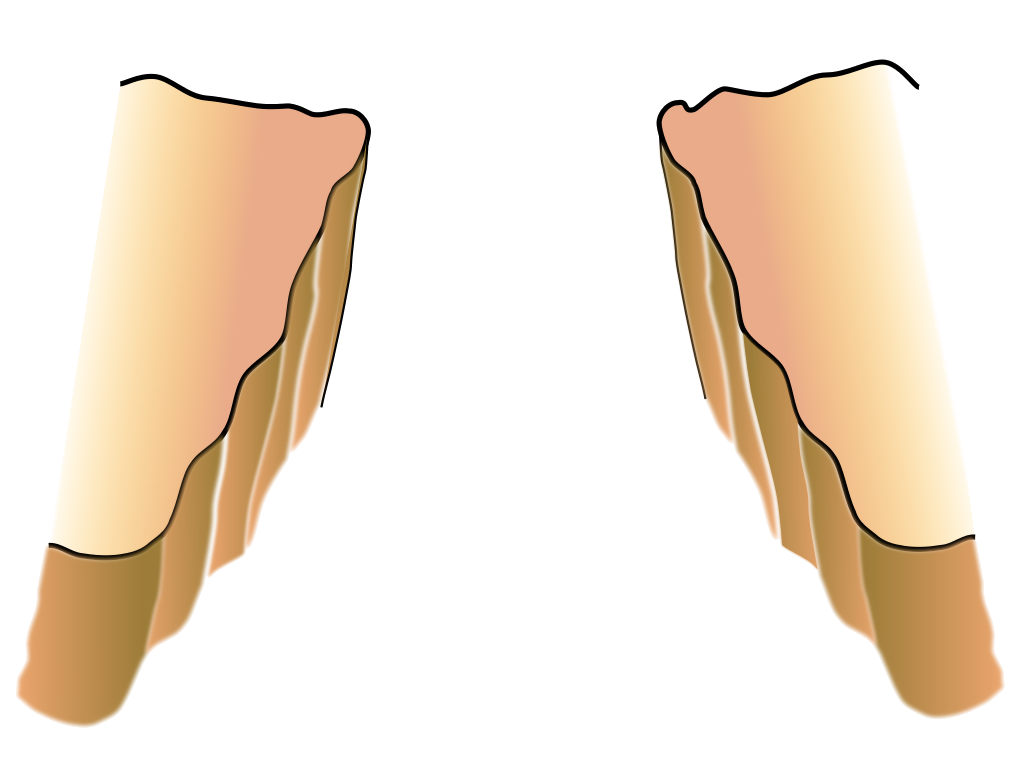
\includegraphics[height=4cm]{../img/chasm.png}}
%
%\only<2->{\hh{Natural Logic} \hspace{3ex} \hh{Lexical Methods} \\}
%\only<2->{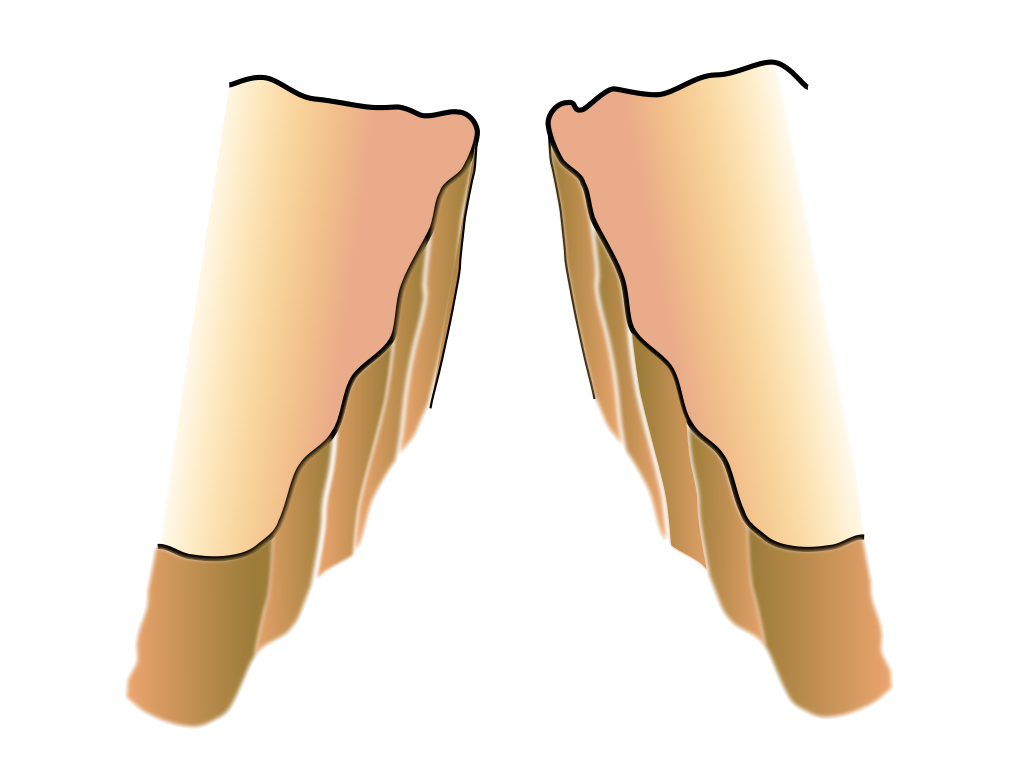
\includegraphics[height=4cm]{../img/chasm-close.png}}
%\end{center}
%\pause
%\pause
%
%\begin{itemize}
%\item Already useful for textual entailment 
%      \cite{key:2008maccartney-natlog,key:2009maccartney-thesis}
%\pause
%\item \hh{This work:} Useful for question answering \newline
%      \hh{This work:} We can bridge the two methods
%\end{itemize}
%
%\only<4->{
%\begin{textblock*}{5cm}(4.5cm,3.5cm)
%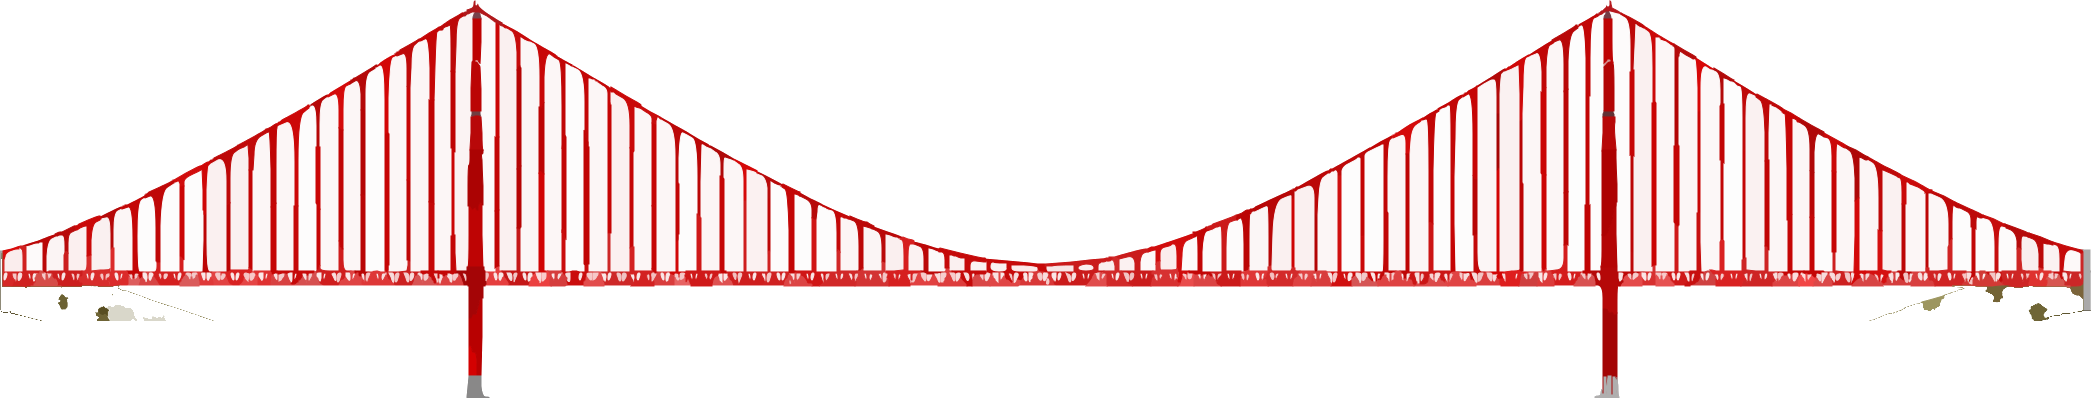
\includegraphics[width=4cm]{../img/golden-gate.png}
%\end{textblock*}
%}
%
%\end{frame}
%
%%
%% Frame 2
%%
%\begin{frame}[noframenumbering]{Future Work}
%\begin{center}
%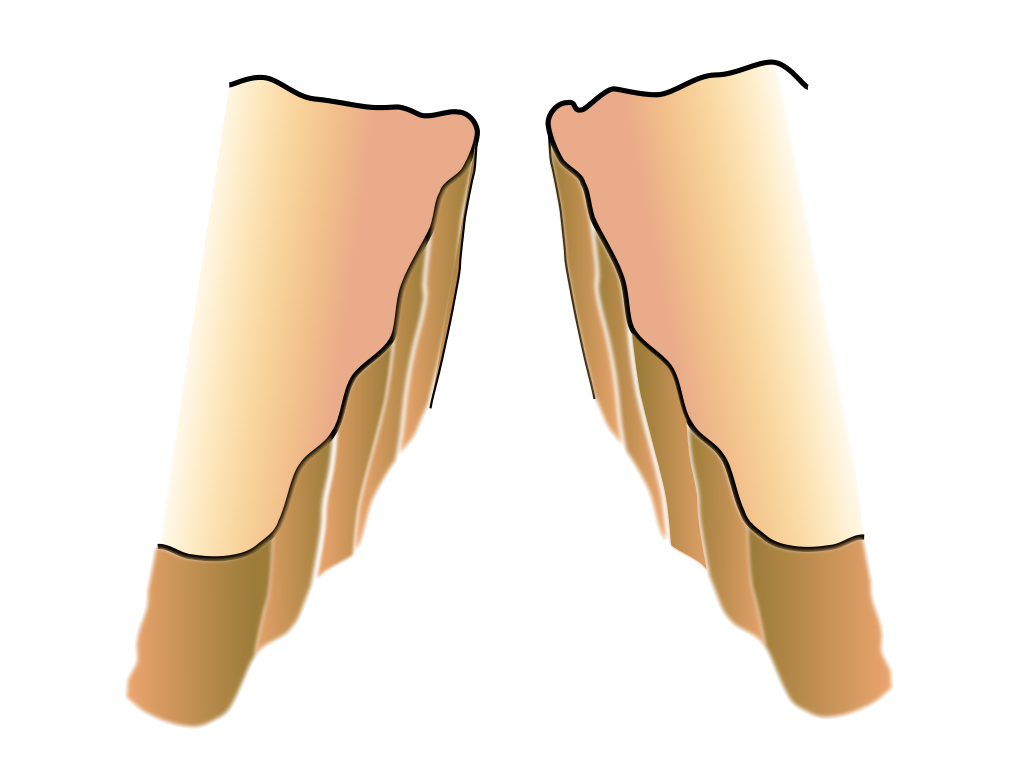
\includegraphics[height=2cm]{../img/chasm-close.png}
%\end{center}
%\vspace{-2ex}
%
%
%\begin{enumerate}
%\item Encode logic in traditionally lexical representations
%  \cite{key:2013bowman-natlog,key:2015bowman-natlog}
%\pause
%\item Make natural logic more expressive
%\pause
%\begin{itemize}
%  \item Propositional + Natural logics: \\
%       \hspace{2ex}\w{Apples are red} $\lor$ \w{\textcolor<4->{darkred}{Bananas are red}} \\
%       \hspace{2ex}\w{\textcolor<4->{darkred}{Bananas are not red}} \\
%       \hspace{0ex}$\therefore$ \w{Apples are red}
%  \pause
%  \pause
%  \item Better handle global syntactic rewrites
%\end{itemize}
%\end{enumerate}
%\end{frame}


%%%%%%%%%%%%%%%%%%%% 
%% Broader Future Work
%%%%%%%%%%%%%%%%%%%% 
%\begin{frame}{Future Work}
%\begin{center}
%\textbf{\w{``The Good Dinosaur was Pixar 's 
%           second best movie in 2015''}}
%\end{center}
%\vspace{2ex}
%
%\begin{itemize}
%\item More to life than QA: leverage knowledge for downstream tasks.
%\pause
%\vspace{2ex}
%\item Domain-generality: Training on new domains adds knowledge; but don't
%      forget old domain!
%\end{itemize}
%\vspace{2ex}
%\pause
%
%\begin{center}
%\hh{Thanks!}
%\end{center}
%\end{frame}



%%%%%%%%%%%%%%%%%%% 
% History of Knowledge
%%%%%%%%%%%%%%%%%%% 
\newcommand{\tabitem}{~~\llap{\textbullet}~~}

\def\title{Going Forward}
\begin{frame}{\title}
\vspace{-3ex}
\begin{center}
\begin{tabular}{ll}
  \multirow{4}{*}{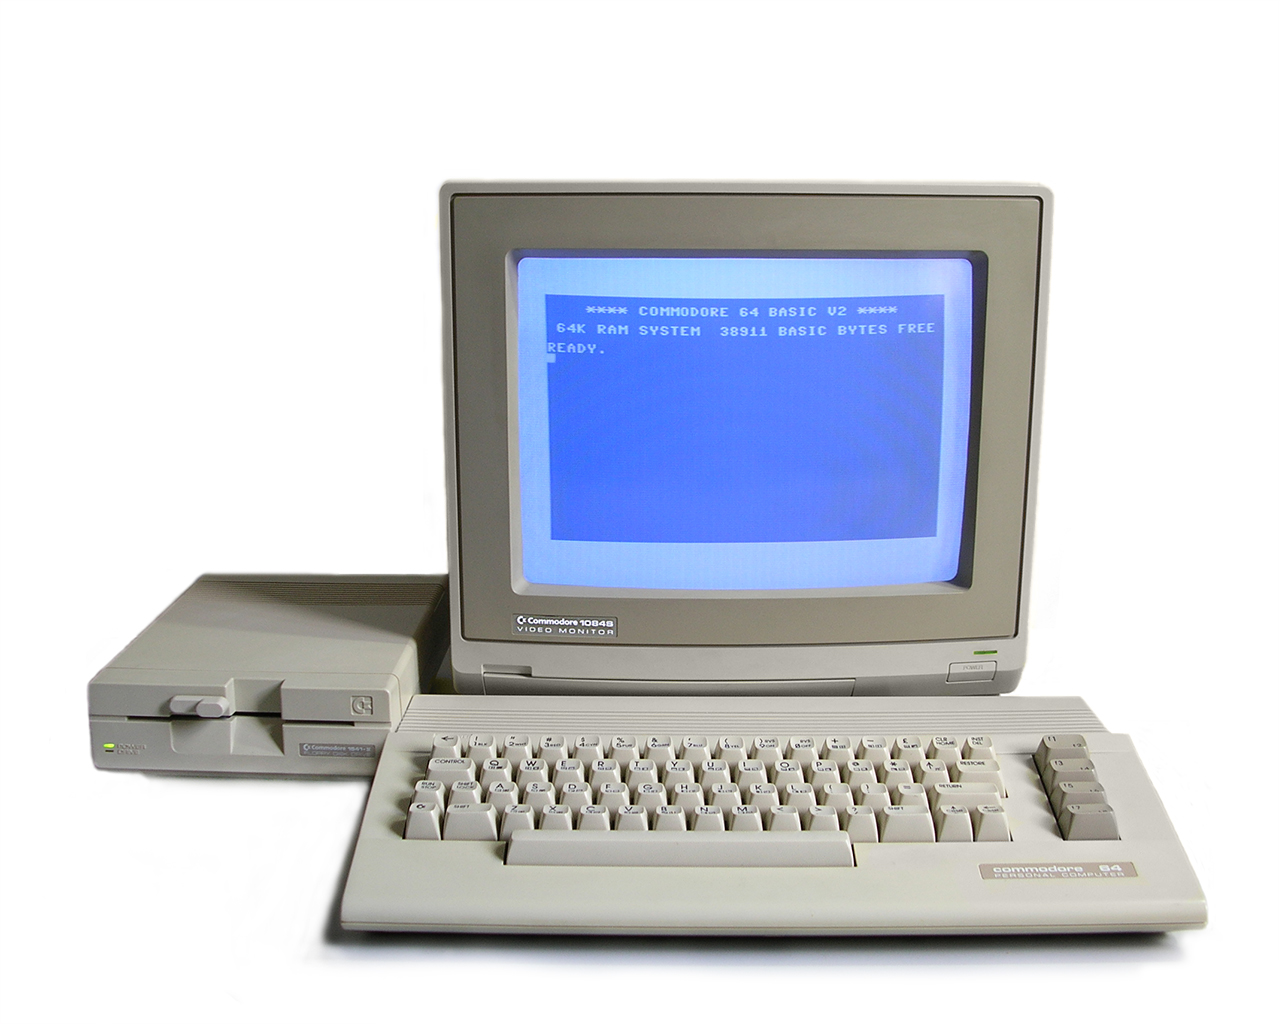
\includegraphics[height=2.0cm]{../img/c64.jpg}} &
    \hh{Before 1990's: Knowledge was a big deal} \\
  & \tabitem Pitiful compute \\
  & \tabitem Pitiful quantities of data (e.g., no internet) \\
  & ~~~~\llap{$\Rightarrow$} Cyc (2.1M facts) \\
  &\\
  \pause
  
  \multirow{4}{*}{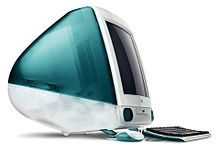
\includegraphics[height=2.0cm]{../img/imac.jpg}} &
    \hh{1990 -- Now: Supervised machine learning} \\
  & \tabitem Lots of compute \\
  & \tabitem Lots of data \\
  \pause
  & ~~~~\llap{$\Rightarrow$} ``Idiot Savants'' \\
  \pause
  &\\
  
  \multirow{5}{*}{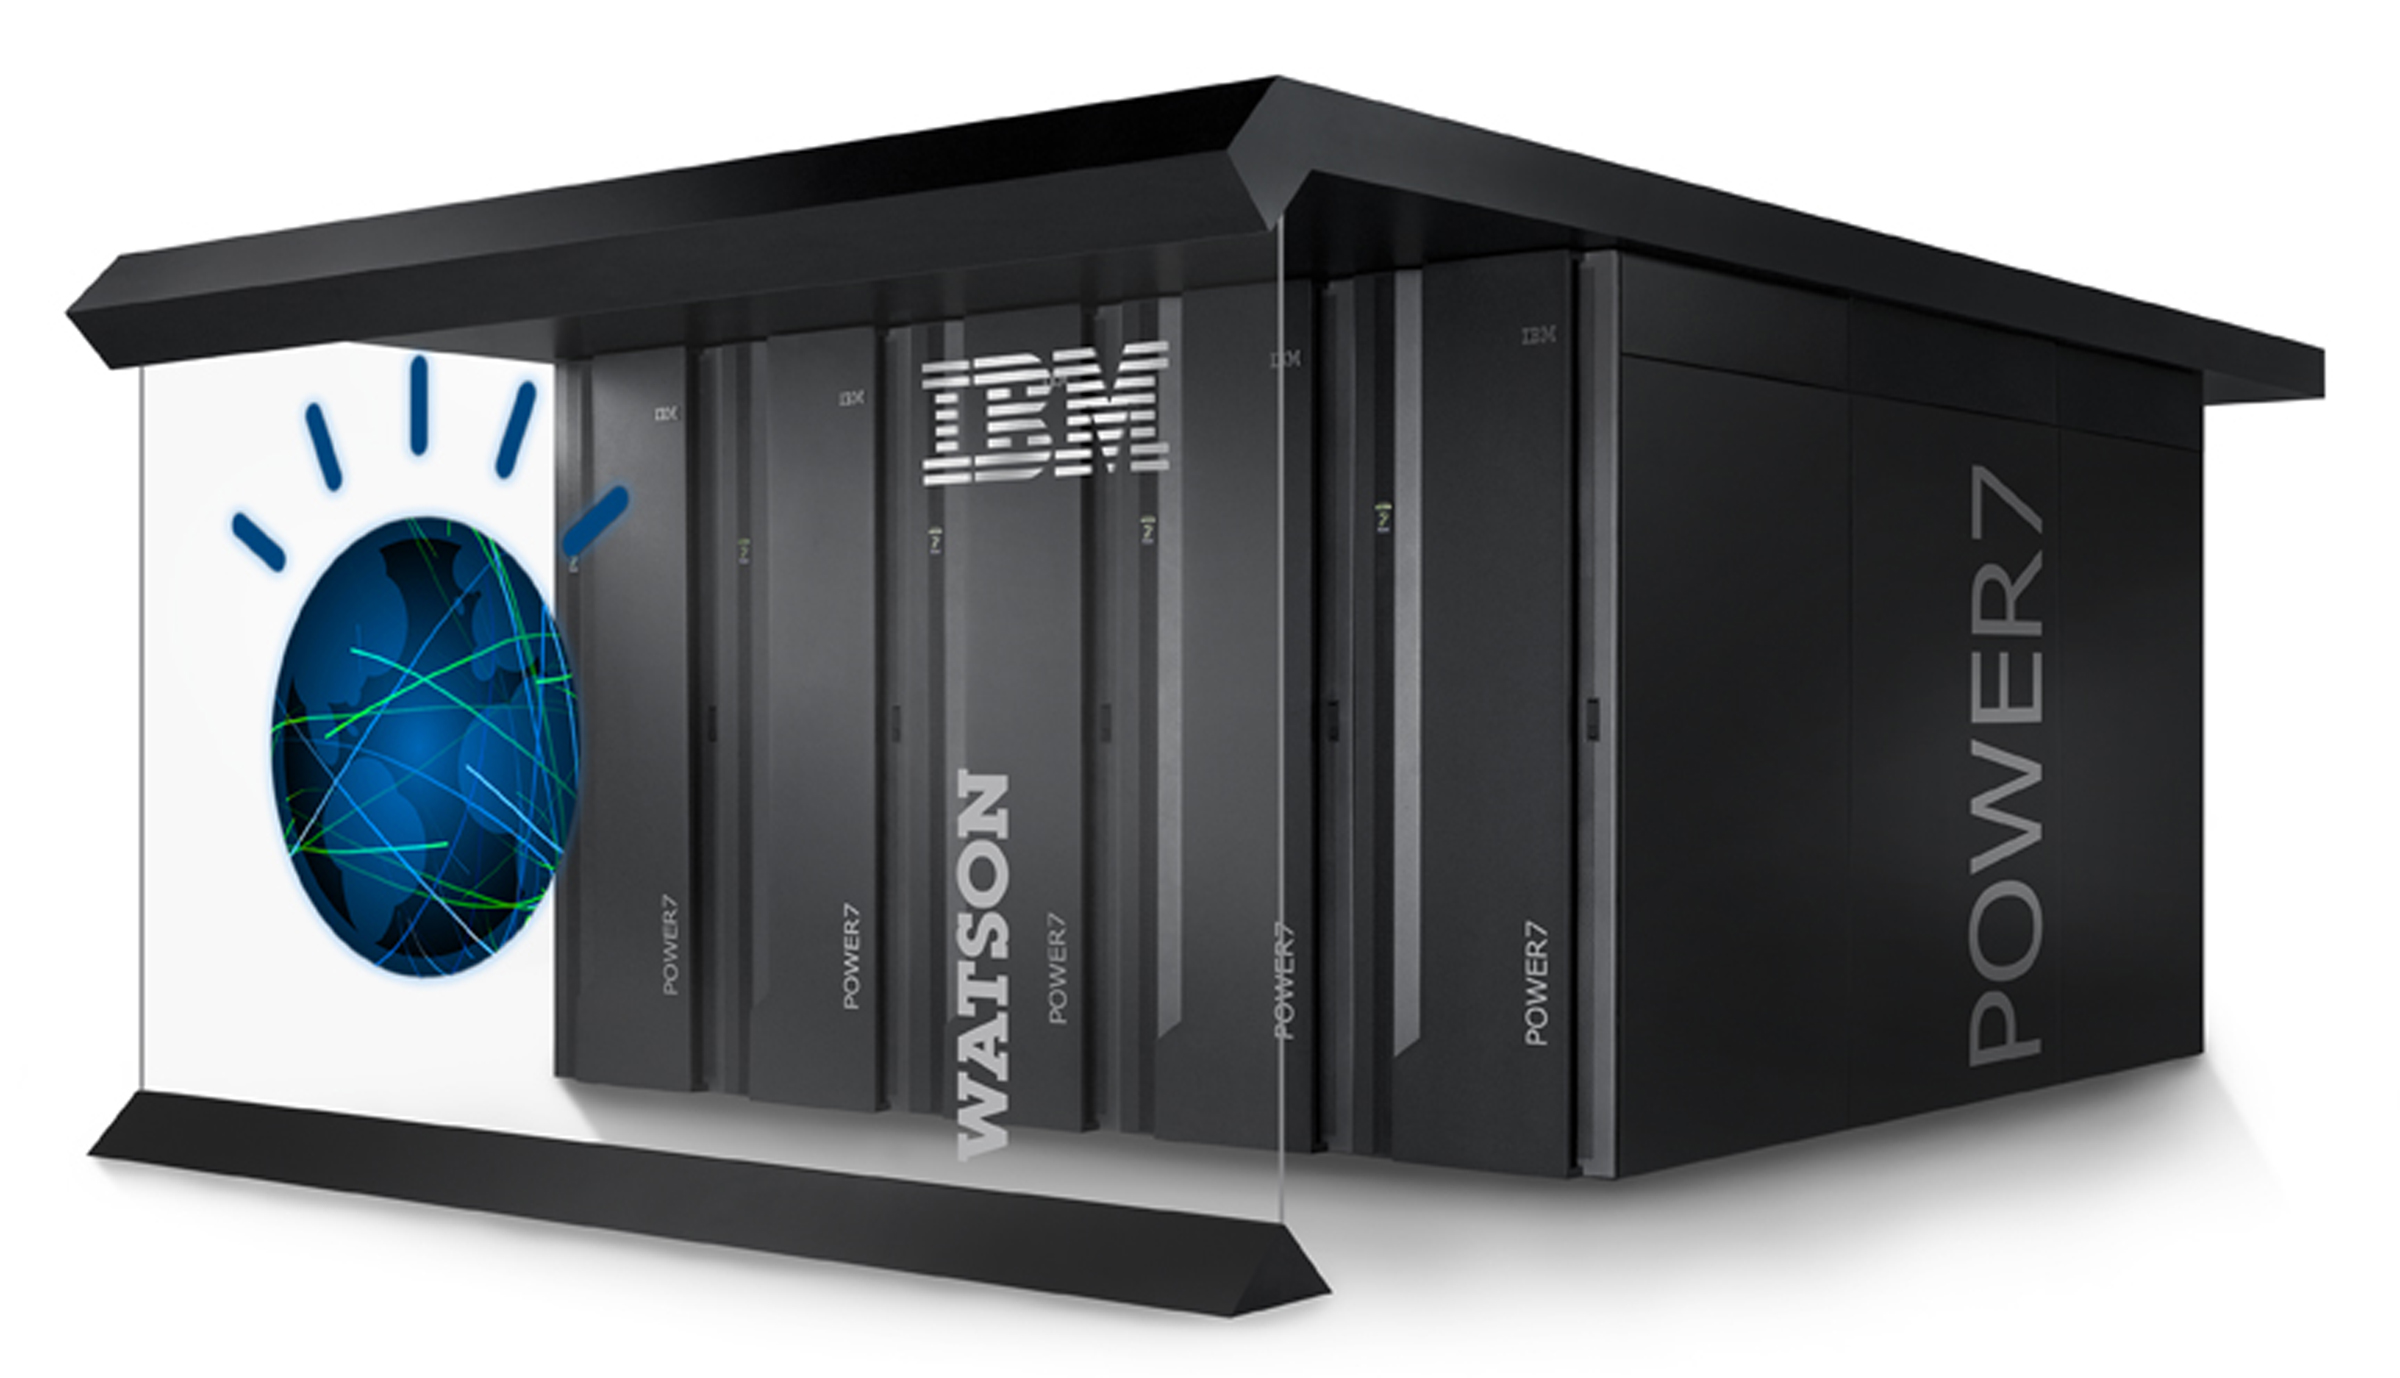
\includegraphics[height=1.75cm]{../img/watson.jpg}} &
    \hh{Future: Open-domain non-factoid knowledge} \\
  & \tabitem Tackle hard science questions \\
  & \tabitem Dialog systems for knowledge acquisition \\
  & \tabitem Reinforcement / ``never ending'' \\
  & ~~~~~ language learning\\
  
\end{tabular}
\end{center}
\end{frame}

